  \documentclass[12pt,oneside]{article}

%%%%%%%%%%%%%%%%%%%%%%%%%%%%
%%   Zusaetzliche Pakete  %%
%%%%%%%%%%%%%%%%%%%%%%%%%%%%
\usepackage{acronym}
\usepackage{enumerate}
\usepackage{a4wide}
\usepackage{fancyhdr}
\usepackage{graphicx}
\usepackage{palatino}
\usepackage{blindtext}
\usepackage{multirow}
\usepackage[ruled,longend]{algorithm2e}
\usepackage{float}
\usepackage{amsmath}
\usepackage{amssymb}
\usepackage{listings}
\usepackage{tocbibind}
\usepackage{dirtytalk}
%folgende Zeile auskommentieren für englische Arbeiten
\usepackage[ngerman]{babel}
 
\usepackage[bookmarks]{hyperref}
\usepackage[T1]{fontenc}
\usepackage[utf8]{inputenc}
\usepackage[a-1b]{pdfx}
\usepackage[justification=centering]{caption}
%\usepackage[style=unsrt,natbib=true,backend=biber]{biblatex}
\usepackage{csquotes}
\usepackage{url}
%\usepackage{subfigure}
\usepackage[utf8]{inputenc}
\usepackage[T1]{fontenc}
% Layout corrections (Schusterjungen)
\clubpenalty = 10000 
% Layout corrections (Hurenkinder) 
\widowpenalty = 10000 
\displaywidowpenalty = 10000

% Figures
\usepackage{caption}
\usepackage[hypcap=true,labelformat=simple]{subcaption}
\renewcommand{\thesubfigure}{(\alph{subfigure})}

% Tables
\usepackage{booktabs} 

\usepackage[backend=biber,style=numeric]{biblatex}
\addbibresource{literatur.bib}


% Newcommand TODO (red in text)
\newcommand{\todo}[1]{\textcolor{red}{TODO: #1}}

% Newcommand TODOM (red at border)
\newcommand{\todom}[1]{\marginpar{\parbox{1.5cm}{\textcolor{red}{TODO:\\ #1}}}}




%%%%%%%%%%%%%%%%%%%%%%%%%%%%%%
%% Definition der Kopfzeile %%
%%%%%%%%%%%%%%%%%%%%%%%%%%%%%%

\pagestyle{fancy}
\fancyhf{}
\cfoot{\thepage}
\setlength{\headheight}{16pt}

%%%%%%%%%%%%%%%%%%%%%%%%%%%%%%%%%%%%%%%%%%%%%%%%%%%%%
%%  Definition des Deckblattes und der Titelseite  %%
%%%%%%%%%%%%%%%%%%%%%%%%%%%%%%%%%%%%%%%%%%%%%%%%%%%%%

\newcommand{\HSFTitle}[8]{

  \thispagestyle{empty}
\begin{center}
    
\includegraphics[width=0.8\textwidth]{logo.eps} \\
    \vspace*{\stretch{1}}
    \end{center}

  %\vspace*{\stretch{1}}
  {\parindent0cm
  \rule{\linewidth}{.7ex}}
  \begin{center}
    \vspace*{\stretch{1}}
    \sffamily\bfseries\Huge
    #1\\
    \vspace*{\stretch{1}}
    \sffamily\bfseries\large
    #3
    \vspace*{\stretch{1}}
  \end{center}
  \rule{\linewidth}{.7ex}

  \vspace*{\stretch{2}}
  \begin{center}
    \Large #2 am #5 der HAW Fulda \\
    \vspace*{\stretch{1}} 
    \large Matrikelnummer:  #4 \\[1mm]
    \large Erstbegutachtung:  #7 \\[1mm]
    \large Zweitbegutachtung:  #8 \\[1mm]
    \vspace*{\stretch{1}}
    \large Eingereicht am #6
  \end{center}
}


%%%%%%%%%%%%%%%%%%%%%%%%%%%%
%%  Beginn des Dokuments  %%
%%%%%%%%%%%%%%%%%%%%%%%%%%%%


\begin{document}
 
 

 \HSFTitle
      {Entwicklung und Implementierung eines Modells zur Erfassung und Bewertung der User Experience am Beispiel der Anwendung eDok des LWV Hessene }        % Titel der Arbeit
      {Bachelorarbeit} % Typ der Arbeit
      {Ali Alkhiami}          % Vor- und Nachname des Autors
      {844620}
      {Fachbereich AI}  % Name des FBs
      {05.mm.yyyy}        % Tag der Abgabe
      {Prof. Dr. Alexander Gepperth}     % Name des Erstgutachters
      {Prof. Dr. Dr. YYY}    % Name des Zweitgutachters

  \clearpage

\lhead{}
    \setcounter{page}{1}
\tableofcontents
%--------------------------------------------------------------------------------------------------------------------------------------------------------------------------------------%
\section{Abkürzungsverzeichnis}
\addcontentsline{toc}{section}{Abkürzungsverzeichnis} % Fügt das Abkürzungsverzeichnis zum Inhaltsverzeichnis hinzu
\begin{acronym}[hyperlinks]
\acro{UX}{User Experience}
\acro{LWV}{Landeswohlfahrtsverband}
\acro{SUS}{System Usability Scale}
\acro{UEQ}{User Experience Questionnaire}
\acro{UI}{User Interface}
\acro{eDok}{elektronische Dokumentenerstellung}
\acro{HCI}{Humin Computer Interaction}
\end{acronym}
%--------------------------------------------------------------------------------------------------------------------------------------------------------------------------------------%
\section{Abstract}
  Diese Arbeit widmet sich der Entwicklung und Implementierung eines Modells zur umfassenden Erfassung und Bewertung der User Experience (UX) am Beispiel der Anwendung eDok des Landeswohlfahrtsverbands Hessen (LWV Hessen).

Da die Bewertung von UX in der Literatur meist durch Surveys, Umfragen und Nutzerbeobachtungen erfolgt, besteht die erste Herausforderung dieser Arbeit darin, Methoden zu implementieren, die es ermöglichen, die UX anhand von Daten zu bewerten, die aus der produktiven Nutzung der Anwendung stammen.

Um dies zu erreichen, werden die messbaren UX-Eigenschaften und -Dimensionen eingehend untersucht, um zu bestimmen, welche Daten sich am besten eignen, wie diese Daten gesammelt werden können und wie die gesammelten Daten zu interpretieren sind.

Innerhalb der Anwendung wurden dazu ein Feedback-Loop und ein Online-Feedback-Fragebogen integriert, über die die Nutzer jederzeit ihr Feedback abgeben können. Zudem werden weitere Faktoren beobachtet, um ein umfassendes Bild der UX zu erhalten.

Zu Beginn der Arbeit wird das Konzept der UX detailliert erläutert, gefolgt von einer kritischen Analyse gängiger Methoden zur UX-Erfassung. Im Mittelpunkt steht die Entwicklung eines Modells, das es ermöglicht, spezifische UX-Aspekte systematisch zu erfassen und zu bewerten.

Das entwickelte Modell zielt darauf ab, eine automatisierte und kontinuierliche Sammlung relevanter Daten sicherzustellen, um daraus fundierte Erkenntnisse über die Nutzererfahrung abzuleiten. Ein besonderer Schwerpunkt liegt dabei auf der Analyse, wie sich die UX durch fortlaufende Weiterentwicklungen und funktionale Erweiterungen der Software verändert.

Des Weiteren wird die technische Umsetzung des Modells beschrieben, einschließlich der Softwarearchitektur und der Implementierung von Mechanismen zur Anonymisierung der erfassten Daten, um den Schutz der Privatsphäre der Nutzer zu gewährleisten. Diese Anonymisierung ist essenziell, um ethischen Standards und datenschutzrechtlichen Vorgaben zu entsprechen.

Die Arbeit schließt mit einer umfassenden Bewertung der Ergebnisse und gibt einen Ausblick auf mögliche Weiterentwicklungen des Modells. Hierbei wird insbesondere auf die Möglichkeit eingegangen, das Modell auf andere behördliche Anwendungen zu übertragen und damit eine breitere Anwendungsperspektive zu eröffnen.

%--------------------------------------------------------------------------------------------------------------------------------------------------------------------------------------%
\section{Einleitung}
Im Bereich der Human-Computer Interaction (HCI) gibt es zwei unterschiedliche Ansätze im Bereich der User Experience (UX): das UX-Design und das User-Centered Design\cite{glanznig}. Letzteres beschäftigt sich mit der Frage, wie ein hochwertiges Produkt gestaltet werden kann, wobei dieser Aspekt jedoch nicht Teil dieser Arbeit ist. Im Fokus steht vielmehr, wie die UX erfasst und gemessen werden kann.\\
In der Literaturrecherche Review hat sich herausgestellt, dass UX  innerhalb einer Anwendung oder sogar für Produkte und Systeme meistens durch Fragebögen oder Nutzerbefragungen bewertet wird. Dabei zeigte sich, dass sich keine der untersuchten Arbeiten mit der automatisierten Bewertung der UX beschäftigt hat.

Es gibt zwar in der Praxis Dienstleistungen, die bestimmte Merkmale der Usability messen und eigenständig bewerten können, jedoch lässt sich die gesamte UX dadurch nicht vollständig erfassen. Eine besondere Herausforderung bei der Bewertung der UX ist die emotionale Ebene. Emotionen durch Zahlen auszudrücken, ohne dabei den Denkprozess der Nutzer oder ihre Mimik zu berücksichtigen, ist durch automatisierte Tools kaum umsetzbar.

In dieser Arbeit wurde auf die Analyse von Mimiken der Nutzer verzichtet. Stattdessen wurden den Nutzern spezifische Aufgaben zur Verfügung gestellt, die über eine Matrix gewichtet wurden, um eine automatisierte Feedback der UX zu implementieren. Da Usability ein Teil der UX ist, der eher pragmatisch ausgerichtet ist und als „Engineer UX“ bezeichnet wird, ist es in gewisser Weise einfacher, diesen Aspekt zu automatisieren.

Das entwickelte Modell hat seine Stärken und Schwächen, die im Detail analysiert werden. Seine Qualität hängt stark von den gesammelten Daten und deren Auswertung ab. Die UX-Bewertung wurde ausschließlich anhand des Nutzerfeedbacks durchgeführt, wobei die Vorerfahrungen und Motivation der Nutzer eine große Rolle spielten – wie es auch bei langfristigen Feldstudien der Fall ist.

Ein Vorteil dieses Modells ist, dass es einen langfristigen Überblick über die UX verschafft und den Frust der Nutzer sichtbar macht. Wenn es Probleme gibt, wissen die Verantwortlichen, wo sie eingreifen müssen. Zudem kann überprüft werden, ob Korrekturen ausreichend waren oder nicht. In diesem Sinne unterstützt das Modell ein nutzerzentriertes Design, bei dem die Wünsche und Beschwerden der Nutzer in den Entwicklungsprozess einfließen.



UX ist ein fortlaufendes Forschungsfeld im Bereich der HCI. Es begann an Bedeutung zu gewinnen, als Anwendungen immer komplexer und anspruchsvoller wurden.\newline

Da immer mehr Menschen digitale Produkte und Dienste nutzen, steigt die Bedeutung von Benutzerfreundlichkeit und einem positiven Nutzererlebnis. Produkte, die sich durch eine intuitive Bedienung und ein ansprechendes Design auszeichnen, setzen sich im Wettbewerb durch und steigern die Nutzerzufriedenheit nachhaltig.\newline

Heutzutage gibt es oft mehrere Softwarelösungen für ein digitales oder reales Problem. Aus diesem Grund spielt UX und Usabilty eine entscheidende Rolle bei der Auswahl eines Produkts. Ein gut gestaltetes Nutzererlebnis kann den Unterschied ausmachen, ob sich Benutzer für eine bestimmte Lösung entscheiden oder zu einem anderen Produkt wechseln.\newline

Die meisten Experten und wissenschaftlichen Arbeiten sind sich einig, dass UX noch ein relativ junges Forschungsfeld ist. Aufgrund der dynamischen und subjektiven Natur des Themas konnte bisher keine einheitliche Definition festgelegt werden. Dies bietet jedoch den Vorteil, das Thema aus verschiedenen Blickwinkeln betrachten zu können und unterschiedliche Meinungen zu berücksichtigen. Dadurch entsteht ein breiteres und tieferes Verständnis für das Konzept der UX, was der weiteren Entwicklung der Disziplin zugutekommt.\newline
Auf der Kehrseite erschweren unterschiedliche Hintergründe und Fachvokabulare den Fortschritt.\cite{glanznig}
 

Hassenzahl und Tractinsky haben in Ihre Arbeit User experience – a research agenda UX  erlautert, dass \say{User Experience ist ein interessantes Phänomen: Es wurde von der HCI-Community schnell angenommen, aber oft kritisiert, da es vage und schwer fassbar ist. Der Begriff umfasst verschiedene Bedeutungen (Forlizzi und Battarbee 2004), von klassischer Usability bis hin zu Schönheit, hedonischen, affektiven und erfahrungsbasierten Aspekten der Technologienutzung\protect \footnote{Eigene Übersetzung}.}\cite{research}\newline




\subsection{Motivation}

Die Nutzung des Internets ist in den letzten Jahren zu einem festen Bestandteil des Alltags der deutschsprachigen Bevölkerung geworden. Laut der ARD/ZDF-Onlinestudie \cite{ard} verwenden mittlerweile rund 90 Prozent der Menschen ab 14 Jahren regelmäßig das Internet, wobei die mediale Internetnutzung im Jahr 2019 besonders stark zugenommen hat.

Diese Entwicklung unterstreicht die zunehmende Relevanz digitaler Medien und stellt neue Anforderungen an die Gestaltung von Nutzererlebnissen. Es wird zunehmend wichtiger, digitale Inhalte und Services so zu gestalten, dass sie den sich wandelnden Ansprüchen der Nutzer gerecht werden. UX spielt eine zentrale Rolle bei der Bewertung und Optimierung von Softwareanwendungen. Dies gilt insbesondere für behördliche Anwendungen wie eDok, das vom LWV Hessen und anderen Institutionen genutzt wird. Hier ist es entscheidend, die UX zu erfassen und zu verbessern, um die Benutzerfreundlichkeit und Effizienz der Anwendung zu steigern.

Eine besondere Herausforderung besteht darin, Bereiche innerhalb der Anwendung zu identifizieren, die ein verbessertes Design oder zusätzliche Informationen erfordern. Oft sind Nutzer unsicher, wie sie ihre Ziele innerhalb der Anwendung erreichen können oder fühlen sich von der Informationsmenge überfordert. Hier setzt das entwickelte Modell an, das die UX automatisiert erfasst und eine fundierte Analyse ermöglicht. So können gezielt Schlüsselaspekte identifiziert werden, die optimiert werden sollten, um die Nutzerzufriedenheit zu steigern.

Vor allem bei komplexen Webanwendungen wie eDok besteht ein großes Bedürfnis, kontinuierlich Feedback von den Nutzer*innen einzuholen, um deren Erfahrungen besser zu verstehen und die Anwendung kontinuierlich zu verbessern. Durch die Implementierung des entwickelten Modells wird es möglich, spezifische UX-Aspekte systematisch zu erfassen und einen umfassenden Überblick über das Nutzererlebnis zu gewinnen.

Zusätzlich führen die regelmäßige Einführung neuer Funktionen und Veränderungen in der Benutzeroberfläche zu einer dynamischen Komplexitätsentwicklung
 in verschiedenen Bereichen der Anwendung. Ein Überblick über die Entwicklung der UX im Laufe der Zeit ermöglicht eine proaktive Anpassung und Optimierung, 
sodass die Anwendung trotz zunehmender Komplexität benutzerfreundlich bleibt.

in dem Papier "User Experience Evaluation Methods in Academic and
Industrial Contexts" wurde drauf hingewiesen, dassUx bemessung und bewertung Methoden 
 ein wichtige Rolle spielen, um sicherzustellen das die Einticklung des Produkts in die Richtige Richtung geht.\cite{Virpi}

Das Modell bietet zudem Einblicke in die Effizienz bestimmter Bereiche der Anwendung und zeigt, wie sich die Komplexität im Laufe der Zeit verändert hat. Wenn eine Seite umfangreiche Änderungen erfahren hat, können die Entwickler*innen durch das Modell schnell nachvollziehen, wie sich UX- und Usability-Aspekte nach der Implementierung verändert haben und ob weitere Verbesserungen erforderlich sind.
%todo auf 15 seiten bringen
\subsection{Ziel der Arbeit}
Das Ziel dieser Arbeit ist es, zentrale Elemente der UX zu identifizieren, rausfinden wir man das bemessen und bewerten kann. 

Ein Modell zu entwickeln, das diese Elemente darstellt, um die UX innerhalb einer Anwendung erfassen und bewerten zu können. Es soll die Vorteile eines solchen Modells aufzeigen.
Die gesammelten Daten sollen anonymisiert werden, und die Ergebnisse des Modells sollen darüber Auskunft geben, wie sich die UX im Verlauf der Anwendungsentwicklung verändert hat. Zudem soll das Modell die UX an verschiedenen Stellen innerhalb der Anwendung erfassen und bewerten können. Entwickler*innen erhalten die Möglichkeit, zusätzliche Stellen zu messen oder solche zu entfernen, die mit der Zeit an Relevanz verloren haben.
\subsection{Fragestellung}
Welche spezifischen, anonymisierten Daten sind erforderlich, um die UX präzise und systematisch zu erfassen? Wie lassen sich diese Daten über Zeiträume hinweg analysieren, um dynamische Veränderungen zu erkennen und gezielte Optimierungsmöglichkeiten der Anwendung zu erschließen?

\section{Über der Landeswohlfahrtsverband Hessen}
Der Landeswohlfahrtsverband Hessen ist eine zentrale Organisation in Hessen, die sich für die soziale Integration und Unterstützung von Menschen mit Behinderungen einsetzt. Der Verband ist überörtlicher Träger der Eingliederungshilfe und fördert unter anderem in den Bereichen Wohnen, Bildung, Mobilität und Arbeit. Mit der Umsetzung des Bundesteilhabegesetzes und weiteren Programmen wie dem Persönlichen Budget  und dem Budget für Arbeit" unterstützt der LWV Hessen die selbstbestimmte Lebensführung und die gesellschaftliche Teilhabe der Betroffenen. Der LWV unterhält zudem Förderangebote für Kinder und Jugendliche, insbesondere für solche mit geistigen, emotionalen oder körperlichen Einschränkungen. Hierzu zählen Frühberatungsstellen, Förderschulen und Angebote zur inklusiven Beschulung. Zusätzlich ist der Verband Ansprechpartner für Menschen, die Leistungen des Sozialen Entschädigungsrechts benötigen.\subsection{Das Anlei-service GmbH}
Die ANLEI-Service GmbH ist eine Tochtergesellschaft des LWV Hessen  und bietet IT-Dienstleistungen für die Sozialverwaltung. Sie entwickelt Systeme zur Unterstützung der Antragsbearbeitung, Leistungsgewährung und Abrechnung von Sozialleistungen, insbesondere in den Bereichen Eingliederungshilfe, Sozialhilfe und Kriegsopferfürsorge. Zu den zentralen Anwendungen zählen das Integrierte Berichtssystem (IBS) für betriebswirtschaftliche Analysen und MASS zur maschinellen Abrechnung mit Einrichtungen und Trägern

\section{Über eDok}
   
eDok Dient als Service für alle aufrufenden Anwendungen zur Erstellung von barrierefreien Dokumenten
Löst das Schriftstück Erstellungssystem (SE) ab, das auf Microsoft Word und Makros basiert und integriert Doxee/Infinica als Subsystem für die Dokumentbearbeitung und Output-Generierung, sodass eine Verwendung sowohl mit Interaktiven Elementen (Bearbeitung des entstehenden Dokuments), als auch im Hintergrund (Dunkelverarbeitung) erfolgen kann
Ziel und Vision von eDok ist es, eine universelle und generelle Schnittstelle für unsere Anwendungen zur einfachen, effizienten und performanten Erstellung von barrierefreien Dokumenten, unter Einbeziehung der Daten aus unseren Fachverfahren, zu bilden
\section{Einführung in das Thema UX}
 
\subsection{was ist UX}
UX ist ein Teilbereich der HCI, der in den frühen 1990er Jahren an Bedeutung gewann \cite{glanznig}. Mit dem Aufkommen neuer Technologien und der zunehmenden Verbreitung digitaler Produkte rückte der Fokus verstärkt auf die Benutzererfahrung und deren Qualität. UX konzentriert sich auf die Interaktion zwischen Mensch und System und zielt darauf ab, Produkte und Anwendungen so zu gestalten, dass sie nicht nur funktional sind, sondern auch emotional ansprechend und benutzerfreundlich.
Die Definition von UX  wurde in der Literatur von verschiedenen Autoren und Organisationen auf vielfältige Weise beschrieben \cite{GOISTAI}.\\


In ihrer Arbeit User Experience – A Research Agenda erläutern Hassenzahl und Tractinsky \cite{research}, dass sich die frühe Forsdchung im Bereich der HCI hauptsächlich auf Verhaltensziele\footnote{Ziele, die Nutzer durch ihr Verhalten erreichen, z.B. die erfolgreiche Bedienung eines Systems in einem Arbeitskontext.} in Arbeitsumgebungen konzentrierte. Dieser Fokus wurde jedoch später durch alternative Ansätze infrage gestellt.\\
In einem frühen Versuch  UX zu definieren, betonte Alben (1996) die Bedeutung von Ästhetik als wesentlichem Qualitätsaspekt von Technologie\footnote{Eigene Übersetzung}\cite{research}.

Hassenzahl  argumentierte, dass interaktive Produkte aus zwei Perspektiven betrachtet werden können: den instrumentellen Aspekten (z.,B. Usability Testing) und den nicht-instrumentellen (hedonischen) Aspekten, die sich auf das emotionale und ästhetische Erleben der Nutzer beziehen \cite{hassenzahl2003}.

 

Die Nielsen Norman Group definiert UX als die Gesamtheit aller Aspekte der Interaktion eines Endnutzers mit einem Unternehmen, seinen Dienstleistungen und Produkten. Hervorgehoben wird, dass herausragende UX nicht nur die spezifischen Bedürfnisse des Nutzers erfüllt, sondern auch durch Einfachheit und Eleganz überzeugt, sodass die Nutzung und der Besitz des Produkts als angenehm empfunden werden. Zudem wird betont, dass eine qualitativ hochwertige UX eine nahtlose Integration verschiedener Disziplinen erfordert, darunter Ingenieurwesen, Marketing, Grafik- und Industriedesign sowie Interface-Design \cite{nngroup}.

Die ISO 9241-210:2019 beschreibt UX als „sämtliche Wahrnehmungen und Reaktionen von Nutzern, die durch die tatsächliche oder erwartete Nutzung eines Systems, Produkts oder einer Dienstleistung hervorgerufen werden“ \cite{ISO}.

Ungeachtet der unterschiedlichen Definitionen herrscht Einigkeit darüber, dass UX das ganzheitliche Erlebnis eines Nutzers mit einem Produkt, einer Dienstleistung oder einem System umfasst. Dabei spielen Faktoren wie Benutzerfreundlichkeit, Emotionen und Zufriedenheit eine zentrale Rolle. In der Literatur werden häufig mehrere Dimensionen von UX hervorgehoben, insbesondere Usability, ästhetische Wahrnehmung, inhaltliche Relevanz und das Vertrauen der Nutzer \cite{toolbox}. Diese Dimensionen sind entscheidend dafür, wie effektiv und zufriedenstellend eine Anwendung wahrgenommen wird und tragen wesentlich zur Gestaltung positiver Nutzererlebnisse bei.

In dem Paper Towards Practical User Experience Evaluation Methods \cite{evaluationmethods} wird darauf hingewiesen, dass die UX-Forschung eine Vielzahl von Modellen und Frameworks entwickelt hat. Diese Modelle adressieren die zentralen Herausforderungen der UX, wie ihre subjektive, kontextabhängige und dynamische Natur sowie die Balance zwischen pragmatischen und hedonischen Aspekten des Nutzererlebnisses. Gleichzeitig wird betont, dass UX zunehmend in der Industrie übernommen wird, die Produktentwicklung jedoch noch immer stark auf traditionellen Usability-Methoden basiert. Die Arbeit unterstreicht die Notwendigkeit praxisnaher UX-Bewertungsmethoden für die Produktentwicklung in der Industrie. Es wird der Schluss gezogen, dass, obwohl die Definition von UX noch weiter verfeinert werden muss, viele Methoden aus der HCI und anderen Disziplinen an die spezifischen Anforderungen der UX-Bewertung angepasst werden können \cite{evaluationmethods}.





Laut \cite{GOISTAI} reicht die bloße Messung von Fehlern, Klicks oder der benötigten Zeit (Usabilty \ref{sec:usability}) nicht aus, um die User Experience (UX) angemessen zu bewerten. Entscheidend ist es, das Erleben des Nutzers vor, während und nach der Verwendung der Anwendung oder des Produkts zu verstehen. Die Entwicklung von Webanwendungen, die Gaming-Industrie sowie der Aufstieg des allgegenwärtigen Computings führten zu einem Paradigmenwechsel, bei dem der Fokus von der reinen Effizienz hin zur Zufriedenheit der Nutzer verlagerte. Dies legte den Grundstein für die Etablierung von UX als eigenständiges Konzept \cite{glanznig}.

\cite{Virpi} argumentiert, dass objektive Messungen, wie die Zeitmessung oder die Erfassung von Fehlern, allein nicht ausreichen, um UX umfassend zu bewerten. Vielmehr sollten auch Emotionen, Erwartungen und die Motivation der Nutzer einbezogen werden. Darüber hinaus ist UX stark kontextabhängig und variiert je nach Einsatzgebiet und Zielgruppe.\\
Zusammenfassend lässt sich sagen, dass UX unterschiedlich interpretiert wurde, jedoch sind sich die meisten Experten einig, dass Usability ein wesentlicher Teil der UX ist. Dennoch geht UX weit über die reine Usability hinaus. Insbesondere die nicht-instrumentellen und hedonischen Aspekte der UX, wie ästhetische Gestaltung, emotionale Reaktionen und das allgemeine Wohlbefinden der Nutzer während der Interaktion, spielen eine zentrale Rolle. UX umfasst somit sowohl funktionale als auch emotionale Dimensionen der Nutzererfahrung.


\subsection{Usability}\label{sec:usability}
\begin{quote} good usability is a precondition for good UX \cite{glanznig}.\end{quote}
Usability bezieht sich auf die funktionalen Aspekte eines Produkts und beschreibt, wie effektiv und produktiv sich das Produkt nutzen lässt. Viele Experten sehen Usability als Teil der UX \cite{GOISTAI}. Während sich Usability auf die Fähigkeit des Nutzers konzentriert, ein System erfolgreich zu nutzen, umfasst UX auch die gesamte Nutzererfahrung und die dabei entstehenden Emotionen.

Die Nielsen Norman Group definiert \cite{nngroup} Usability als ein Qualitätsmerkmal, das bewertet, wie einfach und angenehm eine Benutzeroberfläche zu nutzen ist. Sie umfasst fünf Hauptkomponenten:
\begin{itemize}
    \item \textbf{Erlernbarkeit}: Wie leicht können Benutzer grundlegende Aufgaben beim ersten Mal ausführen?
    \item \textbf{Effizienz}: Wie schnell können Benutzer Aufgaben ausführen, nachdem sie die Schnittstelle gelernt haben?
    \item \textbf{Merkfähigkeit}: Wie einfach können Benutzer ihre Fähigkeiten wiederherstellen, wenn sie das Design nach einer Pause erneut verwenden?
    \item \textbf{Fehlerrate}: Wie viele Fehler machen Benutzer, wie schwerwiegend sind diese und wie leicht können sie sich von ihnen erholen?
    \item \textbf{Zufriedenheit}: Wie angenehm ist die Nutzung der Benutzeroberfläche?
\end{itemize}
Die ISO 9241-210 (2010) definiert die Benutzererfahrung UX und die Gebrauchstauglichkeit (Usability) klar voneinander ab. Während UX sich auf die gesamte Erfahrung und Zufriedenheit der Nutzer bei der Nutzung eines Produkts konzentriert, liegt der Fokus von Usability auf der Effizienz, Effektivität und dem Zufriedenheitsgrad bei der Erledigung konkreter Aufgaben.

Im Kontext einer Webanwendung wie eDok liegt der Schwerpunkt primär auf der Dokumentenerstellung. Es ist wichtig, den Nutzern eine Möglichkeit zu bieten, schnell und effizient Dokumente mit einer gewissen Fehlertoleranz zu erstellen und zu bearbeiten. Im Anschluss daran stellt sich die Frage, wie sich die Nutzer während der Nutzung von eDok fühlen.

 

In diesem Arbeitskontext wird versucht, bestimmte Merkmale der Usability zu messen, zu speichern und zu bewerten.







\subsection{ UX Bewertung}
 
Um geeignete Daten für die Bewertung der UX zu sammeln, müssen zunächst die relevanten Bereiche der UX genauer analysiert werden. Es gilt zu entscheiden, welche Daten sich zur Bewertung der UX eignen und welche sich während der unkontrollierten, produktiven Nutzung der Anwendung erfassen lassen.

In der Literatur wird oft darauf hingewiesen, dass die Wurzeln der UX in der Usability liegen. Dies war der Ausgangspunkt, doch im Laufe der Zeit wurden weitere Faktoren als wichtig erkannt, wie etwa die ästhetische Gestaltung der Anwendung und die emotionale Ebene der Nutzererfahrung. Diese zusätzlichen Aspekte spielen ebenfalls eine wesentliche Rolle bei der umfassenden Bewertung der UX.
 
Um die Usability-Bewertung zu erweitern und die UX detaillierter darzustellen, werden folgende Daten erfasst:

\begin{itemize} \item Benutzerfeedback während der Nutzung (Survey). \item Feedback zu Fehlermeldungen (verständlich, nicht verständlich). \item Bewertung einzelner Prozessschritte zur Zufriedenheitsermittlung (Skala: sehr gut, gut, neutral, unzufrieden, sehr schlecht). \end{itemize}

Laut \cite{GOISTAI} sind UX-Bewertungsmethoden eine Erweiterung der Usability-Messungen. Usability-Bewertung konzentriert sich auf funktionale Aspekte des Systems, während UX-Bewertung zusätzlich die emotionale Dimension und die Erwartungen der Nutzer berücksichtigt.

Das Buch \cite{measuring} beschreibt verschiedene UX-Metriken \footnote{Eine Metrik ist eine Methode, um ein bestimmtes Phänomen oder eine Sache zu messen oder zu bewerten.} zur Erfassung von Nutzeraktionen. Diese Metriken können den Produktverantwortlichen helfen, fundierte Entscheidungen zu treffen.

UX-Metriken ermöglichen eine Bewertung der Interaktion zwischen Nutzer und Produkt in Bezug auf:

\begin{itemize} \item Effektivität (die Fähigkeit, eine Aufgabe zu erfüllen). \item Effizienz (der erforderliche Aufwand zur Aufgabenerfüllung). \item Zufriedenheit (das Maß an Zufriedenheit des Nutzers bei der Aufgabenbewältigung). \end{itemize}


 

\subsection{Messung und Bewertung von Usabilty}
\subsubsection{Messung von Effizienz in eDok}
Prozesse in eDok können verschiedene Status haben, wobei das Ziel in der Regel darin besteht, ein Dokument abzuschließen. Sobald dies erreicht ist, gilt das Hauptziel als erfüllt, obwohl das Dokument auch nach Abschluss noch weiter bearbeitet werden kann.

Der Arbeitsprozess kann jedoch aus unterschiedlichen Gründen unterbrochen werden, wie z.B. durch Fehler oder Internetstörungen. Daher ist der erste Schritt, die Benutzerfreundlichkeit (Usability) zu bewerten und ein klares Endziel der Aufgabe zu definieren. Eine Aufgabe beginnt in der Regel mit der Erstellung und endet mit dem Abschluss. Sobald sie abgeschlossen ist, kann die dafür benötigte Zeit gemessen werden.

Unvollständige Aufgaben in eDok können zu einem späteren Zeitpunkt weiterbearbeitet und abgeschlossen werden. Es ist wichtig, den Zeitpunkt der Unterbrechung und die Wiederaufnahme der Arbeit zu erfassen, um den gesamten Prozessverlauf bis zum Abschluss nachvollziehen zu können.

Nach Abschliessen der Prozess kann dies immernoch bearbeitet werden, dauz ist eigene bessmung für die Aufwand von Bearbeitung, um die Effizanz dazu auch bemessen zu werden.

Die Messungen beschränken sich aus Leistungsgründen auf bestimmte Vorlagen und Prozesse innerhalb der Anwendung, die vom Produktentwicklungsteam festgelegt werden. Zu den erfassten Daten gehören die aufgewendete Zeit, die Häufigkeit der Unterbrechungen sowie die Dauer des gesamten Prozesses von Anfang bis Ende, sowohl mit als auch ohne Unterbrechungen.
\subsubsection{Erfolgsrate}
Fehlern in eDok können aufunterschiedliche Arten auftreten, es gibt Fehlern, die durch bestimmte Nutzer Aktion beseitigt sein können, undefinierte Fehlern, die für die Nutzer verständlich sind und undefinerte Fehler, wo für den Nutzer unbekannt sind, es gibt noch Fehlern die definiert sind aber in der Falsche Stelle aufgeerten sind. Folgende Graph kann die die Fehler klassfizieren.
\begin{figure}[h]
    \centering
    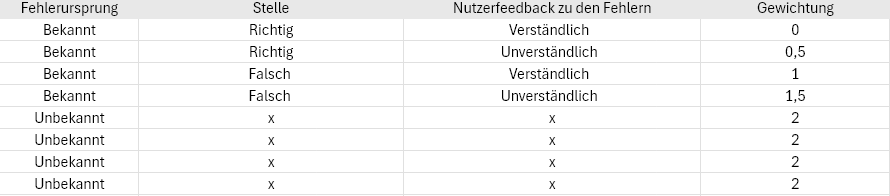
\includegraphics[width=1.00\textwidth]{FehlerMatrix.png}
    \caption{a nice plot}
    \label{fig:mesh1}
\end{figure}

\subsection{Systematische Bewertung weiterer Aspekte der UX}
 Das Modell soll auch weitere Aspekte der UX bewerten. Da die Datensammlung automatisiert erfolgen soll, besteht die Herausforderung darin, herauszufinden, welche Daten Aufschluss über die UX geben, wie diese Daten gesammelt werden können und wie sie zu bewerten sind. In der Praxis wurde die UX häufig durch Nutzerinterviews und Fragebögen bewertet, wobei die Beobachtung der Nutzer und ihrer Interaktionen mit dem Produkt eine wichtige Rolle spielt.

Das Ziel dieser Arbeit ist es jedoch nicht nur, die UX zu bewerten, sondern auch zu untersuchen, wie sie sich im Laufe der Zeit entwickelt. Da sich das Produkt und dessen Funktionen ständig weiterentwickeln, sind Interviews aufgrund von zeitlichen und finanziellen Einschränkungen keine praktikable Lösung.

Eine mögliche Alternative besteht darin, den Nutzern die Möglichkeit oder Aufforderung zu bieten, sich nach der Implementierung neuer Features mit dem Produkt auseinanderzusetzen und Feedback durch einen im Produkt integrierten Fragebogen abzugeben. Darüber hinaus besteht die Möglichkeit, ein allgemeines Feedback über die gesamte Erfahrung mit dem Produkt abzugeben, wobei sich die Struktur der Fragebögen nicht ändert, sondern lediglich deren Umfang variiert.

Die Fragen für das kurzfristige Feedback können von den Entwicklern oder den Produktverantwortlichen angepasst werden, um präzisere Informationen über die aktuelle UX zu erhalten. Diese Flexibilität ermöglicht es, gezielt Fragen zu stellen, die relevante Erkenntnisse über die kurzfristigen Benutzererfahrungen liefern.
 

\subsection{System Usability Scale}
Die SUS wurde von John Brooke in die 1989er erfunden und ist einfach zu nutzen und geeignet für online befragung.
Es sagt nicht wo in der Anwendung es brent, aber es kann dadurch einen Überblick über die gesammte Usabilty innerhalb einer Anwendung sagen.
\subsubsection{Wie sus funktioniert}

\subsection{Messung und Bewertung von Usabilty durch User Behavior}
\begin{itemize}
\item  Clickstream-Analyse: Verfolgt die Klickpfade der Benutzer innerhalb der Anwendung, um herauszufinden, welche Bereiche der Anwendung am häufigsten genutzt werden oder wo Benutzer möglicherweise Schwierigkeiten haben.
\item  Heatmaps: Visualisiert, wo Benutzer auf dem Bildschirm klicken oder ihre Maus bewegen. So kann man sehen, welche Bereiche die meiste Aufmerksamkeit erhalten.
\item  Session-Replay: Aufzeichnung von Benutzersitzungen, um das Verhalten der Benutzer detailliert zu analysieren, z.B. welche Schritte sie bei der Navigation durch die Anwendung unternehmen.
\end{itemize}



\subsection{Was das Modul misst und darstellt}

Das Modul erfasst und stellt folgende Daten dar:

\begin{itemize} 
\item Heatmaps zur Visualisierung von Nutzerinteraktionen.
 \item Klickpositionen und -häufigkeiten.
\item Feedback zu Fehlermeldungen (Like/Dislike, Verständnis der Fehlermeldung). 
\item Emotion-Feedback in Form von Emojis (gut, zufrieden, neutral, unzufrieden, schlecht) mit optionalen Kommentaren.
 \item Fehlerzähler, um die häufigsten Fehler zu identifizieren.
 \item Erfassung der Prozessschritte, bei denen die meisten Nutzer scheitern.
 \item Zeitaufwand pro Prozess, Verweildauer auf einer Seite, Zeit zur Fehlerbehebung, Prozessabbruch und Wiederaufnahme. 
\item Analyse der Prozesse mit der längsten Bearbeitungsdauer.
 \item Usability-Score und UX-Zusammenfassung über einen bestimmten Zeitraum. 
\end{itemize}
 

  
 
%--------------------------------------------------------------------------------------------------------------------------------------------------------------------------------------%
\section{Anonymisierte Erfassung und Behandlung der Daten}
\section{Bedeutung der Anonymisierung}
Bei der Erfassung von UX-Daten ist es entscheidend, dass die Daten anonymisiert werden, um die Privatsphäre der Nutzer*innen zu schützen und ethische Standards einzuhalten.
%--------------------------------------------------------------------------------------------------------------------------------------------------------------------------------------%
\section{Methoden zur Anonymisierung}
\begin{itemize}
\item \textbf{Pseudonymisierung}: Ersatz von personenbezogenen Daten durch Pseudonyme, sodass die Identität der Nutzer*innen nicht direkt ermittelt werden kann.
\item \textbf{Aggregation}: Zusammenfassung der Daten auf eine Ebene, die keine Rückschlüsse auf Einzelpersonen zulässt.
\end{itemize}
%--------------------------------------------------------------------------------------------------------------------------------------------------------------------------------------%
\section{Umsetzung der Anonymisierung bei eDok}
Hier wird beschrieben, wie die Anonymisierung der erhobenen UX-Daten in der Anwendung eDok umgesetzt werden kann, um den Datenschutzbestimmungen zu entsprechen.
\section{Modellarchitektur}
 
\section{Modellimplementierung}
 
\section{Schlussfolgerung und Ausblick}
 
%--------------------------------------------------------------------------------------------------------------------------------------------------------------------------------------%
 
 
  
\printbibliography
 

\end{document}

